% Options for packages loaded elsewhere
\PassOptionsToPackage{unicode}{hyperref}
\PassOptionsToPackage{hyphens}{url}
%
\documentclass[
  10pt,
  ignorenonframetext,
]{beamer}
\usepackage{pgfpages}
\setbeamertemplate{caption}[numbered]
\setbeamertemplate{caption label separator}{: }
\setbeamercolor{caption name}{fg=normal text.fg}
\beamertemplatenavigationsymbolsempty
% Prevent slide breaks in the middle of a paragraph
\widowpenalties 1 10000
\raggedbottom
\setbeamertemplate{part page}{
  \centering
  \begin{beamercolorbox}[sep=16pt,center]{part title}
    \usebeamerfont{part title}\insertpart\par
  \end{beamercolorbox}
}
\setbeamertemplate{section page}{
  \centering
  \begin{beamercolorbox}[sep=12pt,center]{part title}
    \usebeamerfont{section title}\insertsection\par
  \end{beamercolorbox}
}
\setbeamertemplate{subsection page}{
  \centering
  \begin{beamercolorbox}[sep=8pt,center]{part title}
    \usebeamerfont{subsection title}\insertsubsection\par
  \end{beamercolorbox}
}
\AtBeginPart{
  \frame{\partpage}
}
\AtBeginSection{
  \ifbibliography
  \else
    \frame{\sectionpage}
  \fi
}
\AtBeginSubsection{
  \frame{\subsectionpage}
}
\usepackage{amsmath,amssymb}
\usepackage{lmodern}
\usepackage{iftex}
\ifPDFTeX
  \usepackage[T1]{fontenc}
  \usepackage[utf8]{inputenc}
  \usepackage{textcomp} % provide euro and other symbols
\else % if luatex or xetex
  \usepackage{unicode-math}
  \defaultfontfeatures{Scale=MatchLowercase}
  \defaultfontfeatures[\rmfamily]{Ligatures=TeX,Scale=1}
\fi
% Use upquote if available, for straight quotes in verbatim environments
\IfFileExists{upquote.sty}{\usepackage{upquote}}{}
\IfFileExists{microtype.sty}{% use microtype if available
  \usepackage[]{microtype}
  \UseMicrotypeSet[protrusion]{basicmath} % disable protrusion for tt fonts
}{}
\makeatletter
\@ifundefined{KOMAClassName}{% if non-KOMA class
  \IfFileExists{parskip.sty}{%
    \usepackage{parskip}
  }{% else
    \setlength{\parindent}{0pt}
    \setlength{\parskip}{6pt plus 2pt minus 1pt}}
}{% if KOMA class
  \KOMAoptions{parskip=half}}
\makeatother
\usepackage{xcolor}
\newif\ifbibliography
\setlength{\emergencystretch}{3em} % prevent overfull lines
\providecommand{\tightlist}{%
  \setlength{\itemsep}{0pt}\setlength{\parskip}{0pt}}
\setcounter{secnumdepth}{-\maxdimen} % remove section numbering
\usepackage{booktabs}

\usepackage{color, colortbl}
\definecolor{Gray}{gray}{0.9}

\def\begincols{\begin{columns}}
\def\begincol{\begin{column}}
\def\endcol{\end{column}}
\def\endcols{\end{columns}}

\setbeamertemplate{caption}[numbered]
\setbeamertemplate{itemize items}[default]
\setbeamertemplate{itemize subitem}[circle]

\logo{
\includegraphics[scale=0.06]{bbk_side}}
%\usetheme{Madrid}
%\usefonttheme{serif}

%\pgfdeclareimage[scale=0.2]{logo}{bbk2}
%\logo{\pgfuseimage{logo}}

% \begincols
% \begincol{.48\textwidth}
% \endcol
% \begincol{.48\textwidth}
% \endcol
% \endcols

% How many criminal candidates were there? Where and when?
% 6,499 out of 35,075 contesting candidates -- close to 20\%

% Did criminal candidates win elections? Where and when?
% Given that a candidate is a criminal, the probability of winning the election is about 0.22; in contrast, Given that a candidate is NOT a criminal, the probability of winning the election is about 0.12. (X)

% How many criminal politicians were there? Where and when? 

% Party affiliations: BJP (23\%), Congress (18\%), 
\ifLuaTeX
  \usepackage{selnolig}  % disable illegal ligatures
\fi
\IfFileExists{bookmark.sty}{\usepackage{bookmark}}{\usepackage{hyperref}}
\IfFileExists{xurl.sty}{\usepackage{xurl}}{} % add URL line breaks if available
\urlstyle{same} % disable monospaced font for URLs
\hypersetup{
  hidelinks,
  pdfcreator={LaTeX via pandoc}}

\title{\hfill\break
\hfill\break
Investigating the Social World\\
\strut \\}
\author{Week 1: Welcome to the Club\\}
\date{}

\begin{document}
\frame{\titlepage}

\begin{frame}
\begin{center}
\textbf{Lecture 1: Welcome to Investigating the Social World}
\end{center}
\vspace{0.7cm}

\begin{center}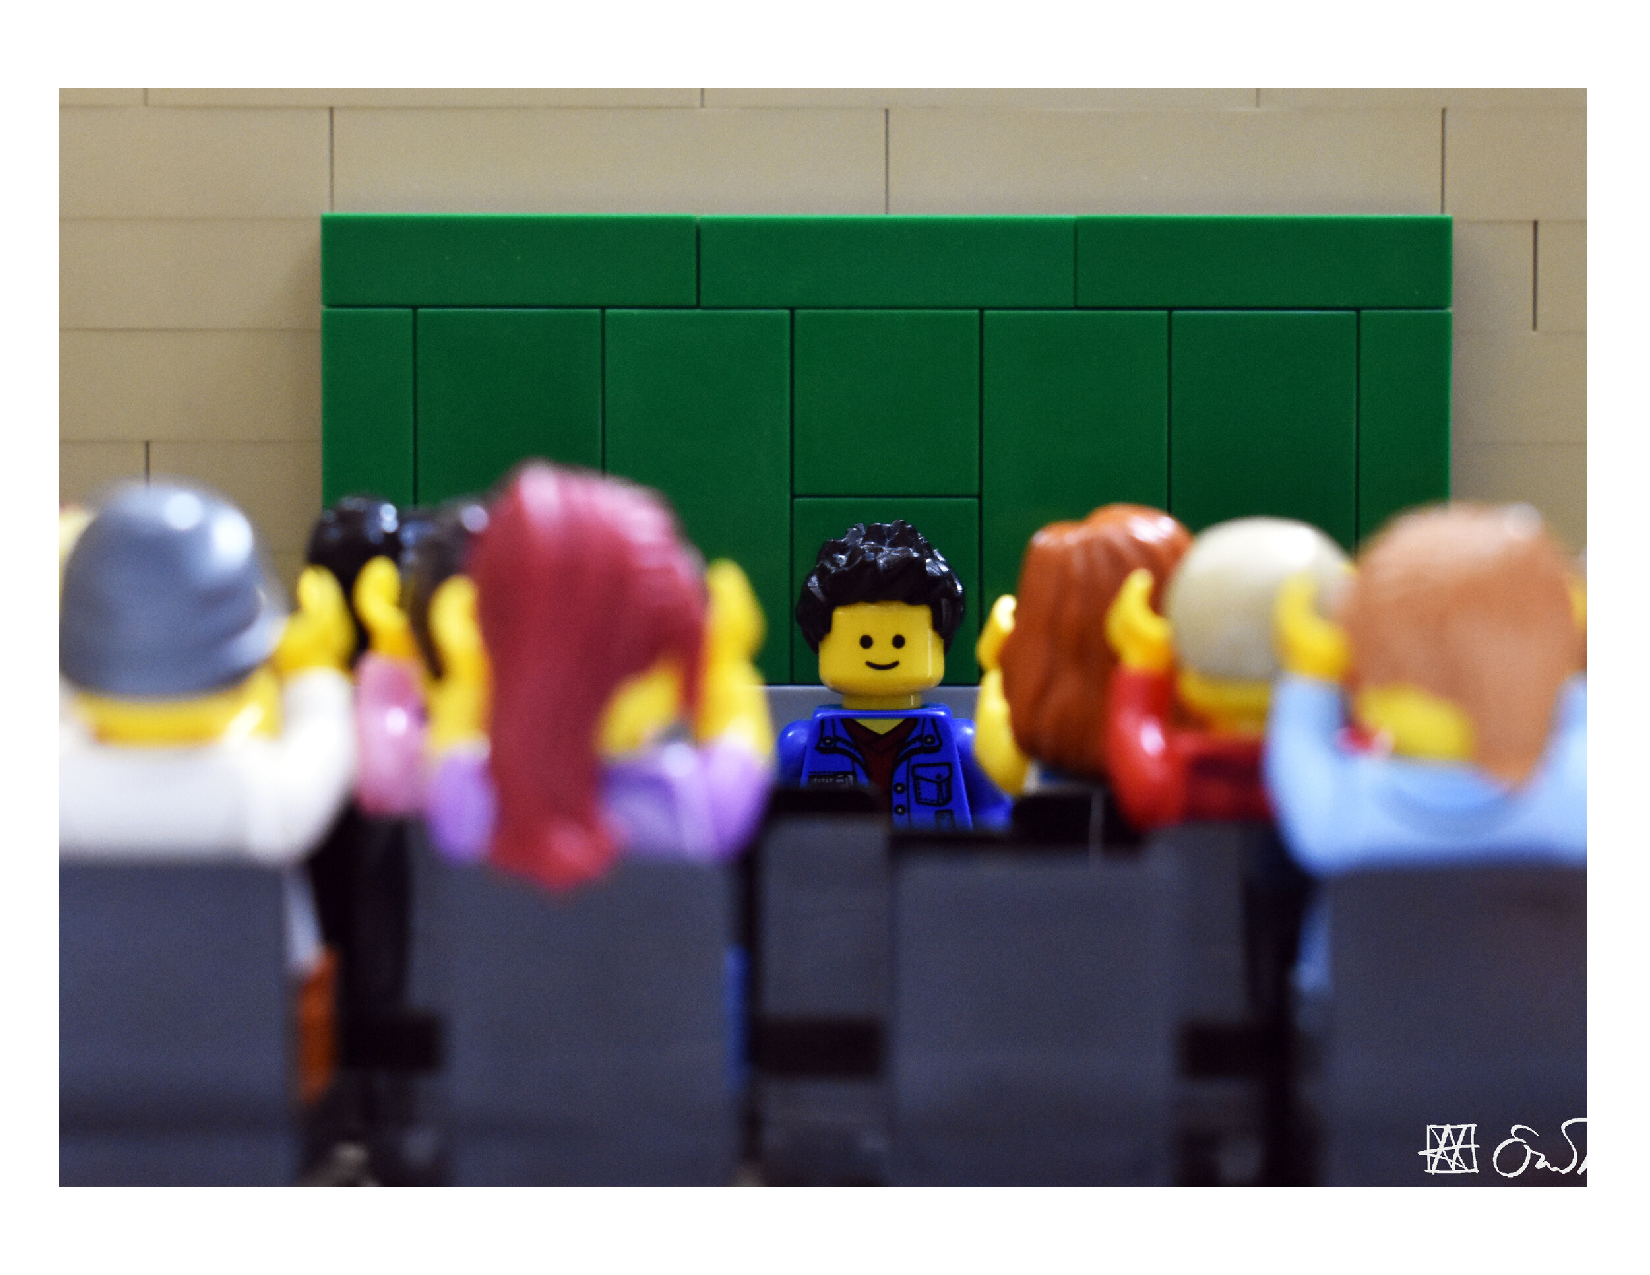
\includegraphics[width=0.7\linewidth]{Figs/cover} \end{center}
\end{frame}

\begin{frame}{Today's plan}
\protect\hypertarget{todays-plan}{}
\begin{itemize}
  \item Introduction: Welcome to the club
  \vspace{0.1cm}
    \begin{itemize}
    \item Module organization
    \item Weekly syllabus and roadmap
    \item Assessment
    \item Student support
    \item Ground rules and tips
    \item Tell us more about you
    \end{itemize}
  \vspace{0.3cm}
  \item Lecture and discussion: What makes "good" social science research?
  \vspace{0.3cm}
  \item Conclusion: "Investigating the social world as a vocation"
\end{itemize}
\end{frame}

\begin{frame}{Module organization}
\protect\hypertarget{module-organization}{}
\vspace{0.2cm}

\begin{center}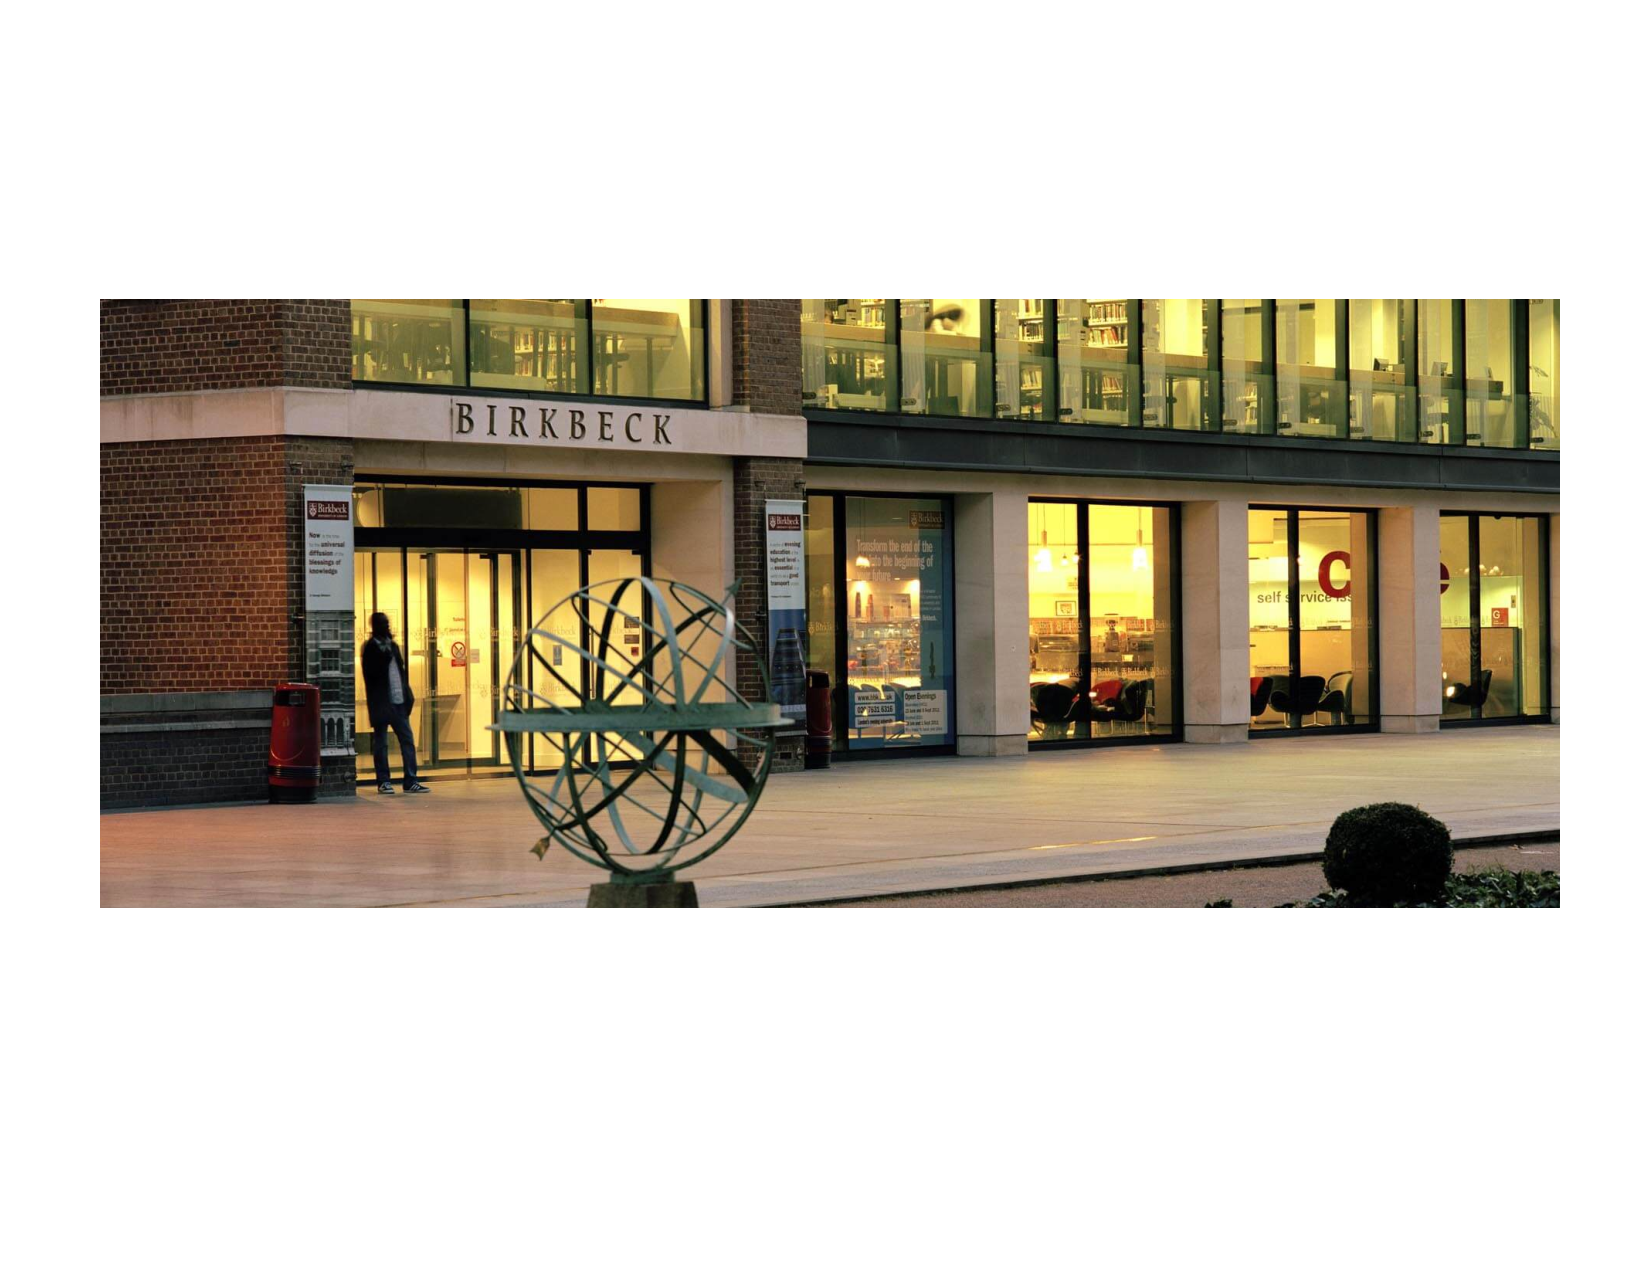
\includegraphics[width=0.8\linewidth]{Figs/bbk_night} \end{center}
\vspace{0.3cm}
\begin{itemize}
\small
  \item When: Every Wednesday, 6-8:30pm
  \item Where: Room G08, Birkbeck Central
  \item Meeting formats
  \begin{itemize}
    \item In-person or recorded lectures
    \item Seminar discussions
  \end{itemize}
\end{itemize}
\end{frame}

\begin{frame}{Weekly syllabus and roadmap}
\protect\hypertarget{weekly-syllabus-and-roadmap}{}
\begin{itemize}
\small
  \item \textbf{Weeks 1-5: Varieties of social research}
  \vspace{0.1cm}
  \begin{itemize}
    \item Theory in social research
    \item Epistemology and theory-empirics alignment
    \item Using numbers to study the social world
    \item Comparative and intl research
  \end{itemize}
  \vspace{0.3cm}
  \item \textbf{Weeks 6-10: Analytical frameworks}
  \vspace{0.1cm}
  \begin{itemize}
    \item Rational choice theory
    \item Psychosocial framing
    \item Decolonizing social research
    \item Intersectional sensibilities
    \item Situating lived experience
  \end{itemize}
\end{itemize}
\end{frame}

\begin{frame}
\vspace{0.2cm}

\begin{center}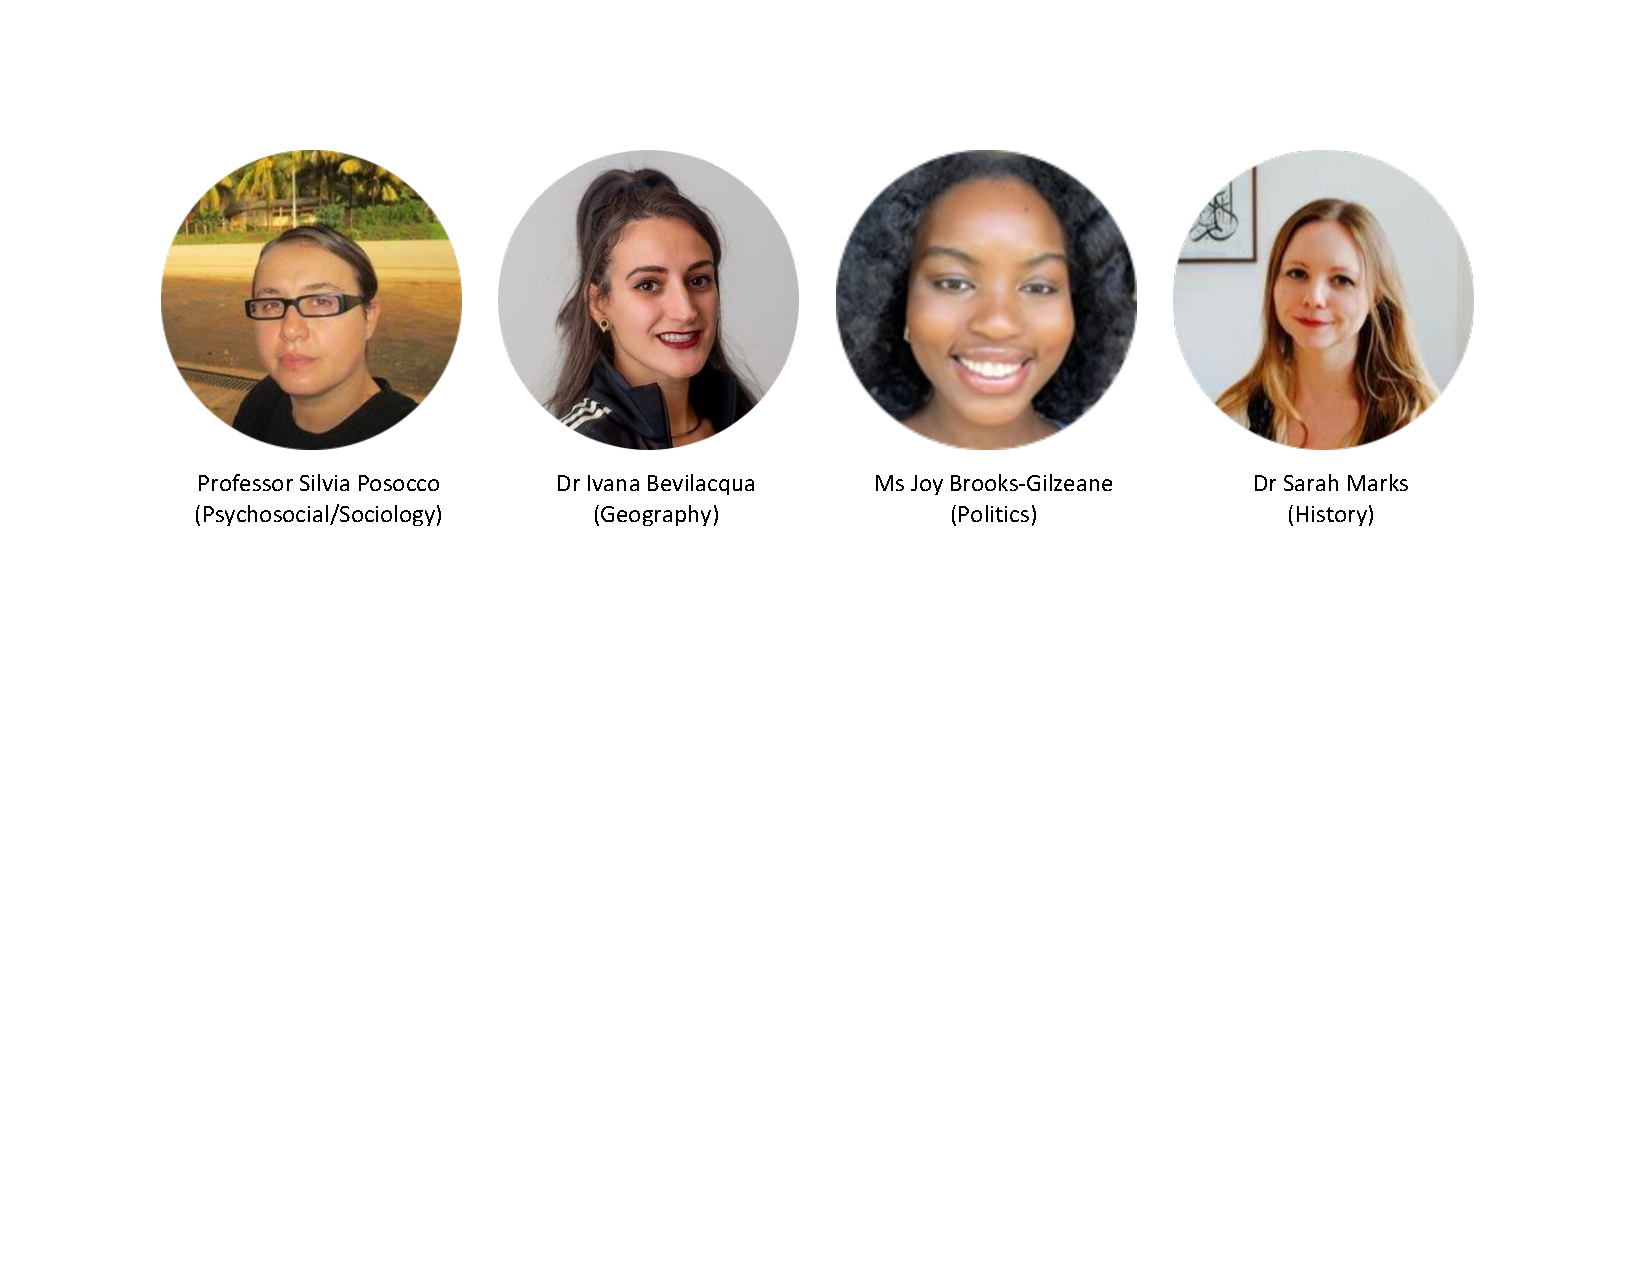
\includegraphics[width=1\linewidth]{Figs/guest} \end{center}
\vspace{0.5cm}
\begin{itemize}
  \item Rational choice theory (Dr Chao-Yo Cheng)
  \item Psychosocial framing (Professor Silvia Posocco)
  \item Decolonizing social research (Dr Ivana Bevilacqua)
  \item Intersectional sensibilities (Ms Joy Brooks-Gilzeane)
  \item Situating lived experience (Dr Sarah Marks)
\end{itemize}
\end{frame}

\begin{frame}{Assessment}
\protect\hypertarget{assessment}{}
\begin{itemize}
  \item Critical methodological review (40\%)
  \vspace{1cm}
  \item Analytical essay (60\%)
\end{itemize}
\end{frame}

\begin{frame}{Assessment}
\protect\hypertarget{assessment-1}{}
\begin{itemize}
  \item Critical methodological review (40\%)
  \vspace{0.1cm}
  \begin{itemize}
    \item Examine a published \textbf{peer-reviewed} article
    \item Answer \textbf{three} questions; write up to \textbf{500 words} (max) for each response
    \item More will be discussed in \textbf{Week 5}
    \item Due on \textbf{April 3 2025}
  \end{itemize}
  \vspace{0.7cm}
  \item Analytical essay (60\%)
\end{itemize}
\end{frame}

\begin{frame}{Assessment}
\protect\hypertarget{assessment-2}{}
\begin{itemize}
  \item Critical mmethodological review (40\%)
  \vspace{0.7cm}
  \item Analytical essay (60\%)
  \vspace{0.1cm}
  \begin{itemize}
    \item Write a 2,500-word essay (max)
    \item Compare two analytical frameworks to analyze a social science phenomenon
    \item More will be discussed in \textbf{Week 6}
    \item Due on \textbf{April 21 2025}
  \end{itemize}
\end{itemize}
\end{frame}

\begin{frame}{Is the module right for you?}
\protect\hypertarget{is-the-module-right-for-you}{}
\begin{itemize}
  \item MSc/PgDip Social Research
  \vpsace{1cm}
  \item MA Sociology (or Psychosocial Studies)
  \vpsace{1cm}
  \item All other subject areas
\end{itemize}
\end{frame}

\begin{frame}{Student support}
\protect\hypertarget{student-support}{}
\begincols
  \begincol{.4\textwidth}
    \vspace{0.4cm}
    \begin{figure}
    \centering
    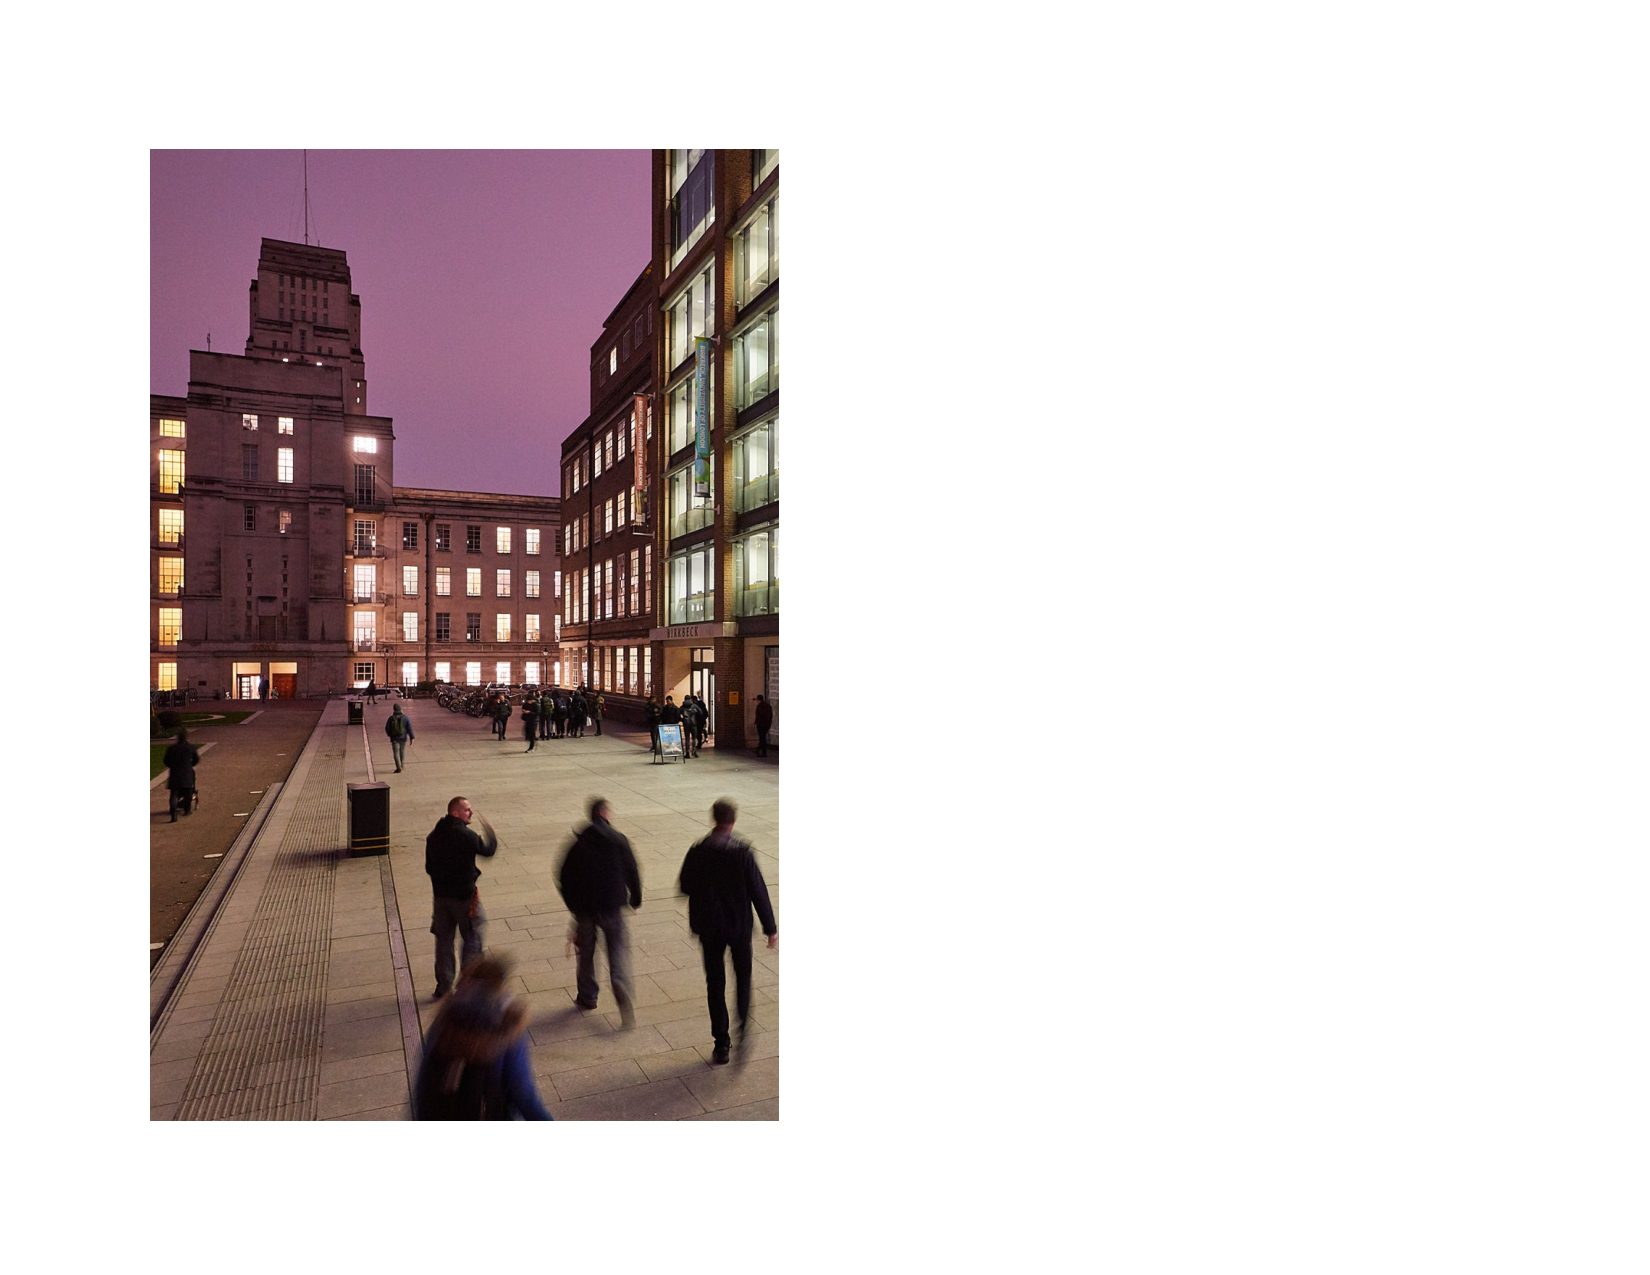
\includegraphics[scale=0.43]{Figs/head}
    \end{figure}
  \endcol
  \begincol{.5\textwidth}
  \hspace{0.2cm}
  \small

\noindent \textbf{Module convenor} \vspace{0.1cm}

\begin{itemize}
    \item Office hours (Friday 3-5pm)
    \item \url{c.cheng@bbk.ac.uk}
  \end{itemize}
  \vspace{0.5cm}

\noindent \textbf{Module administration} \vspace{0.1cm}

\begin{itemize}
    \item Ask (\url{https://www.bbk.ac.uk/ask})
    \item \url{fhss-edu-sss@bbk.ac.uk}
  \end{itemize}
  \vspace{0.5cm}

\noindent \textbf{Student Services} \endcol \endcols
\end{frame}

\begin{frame}
\begin{center}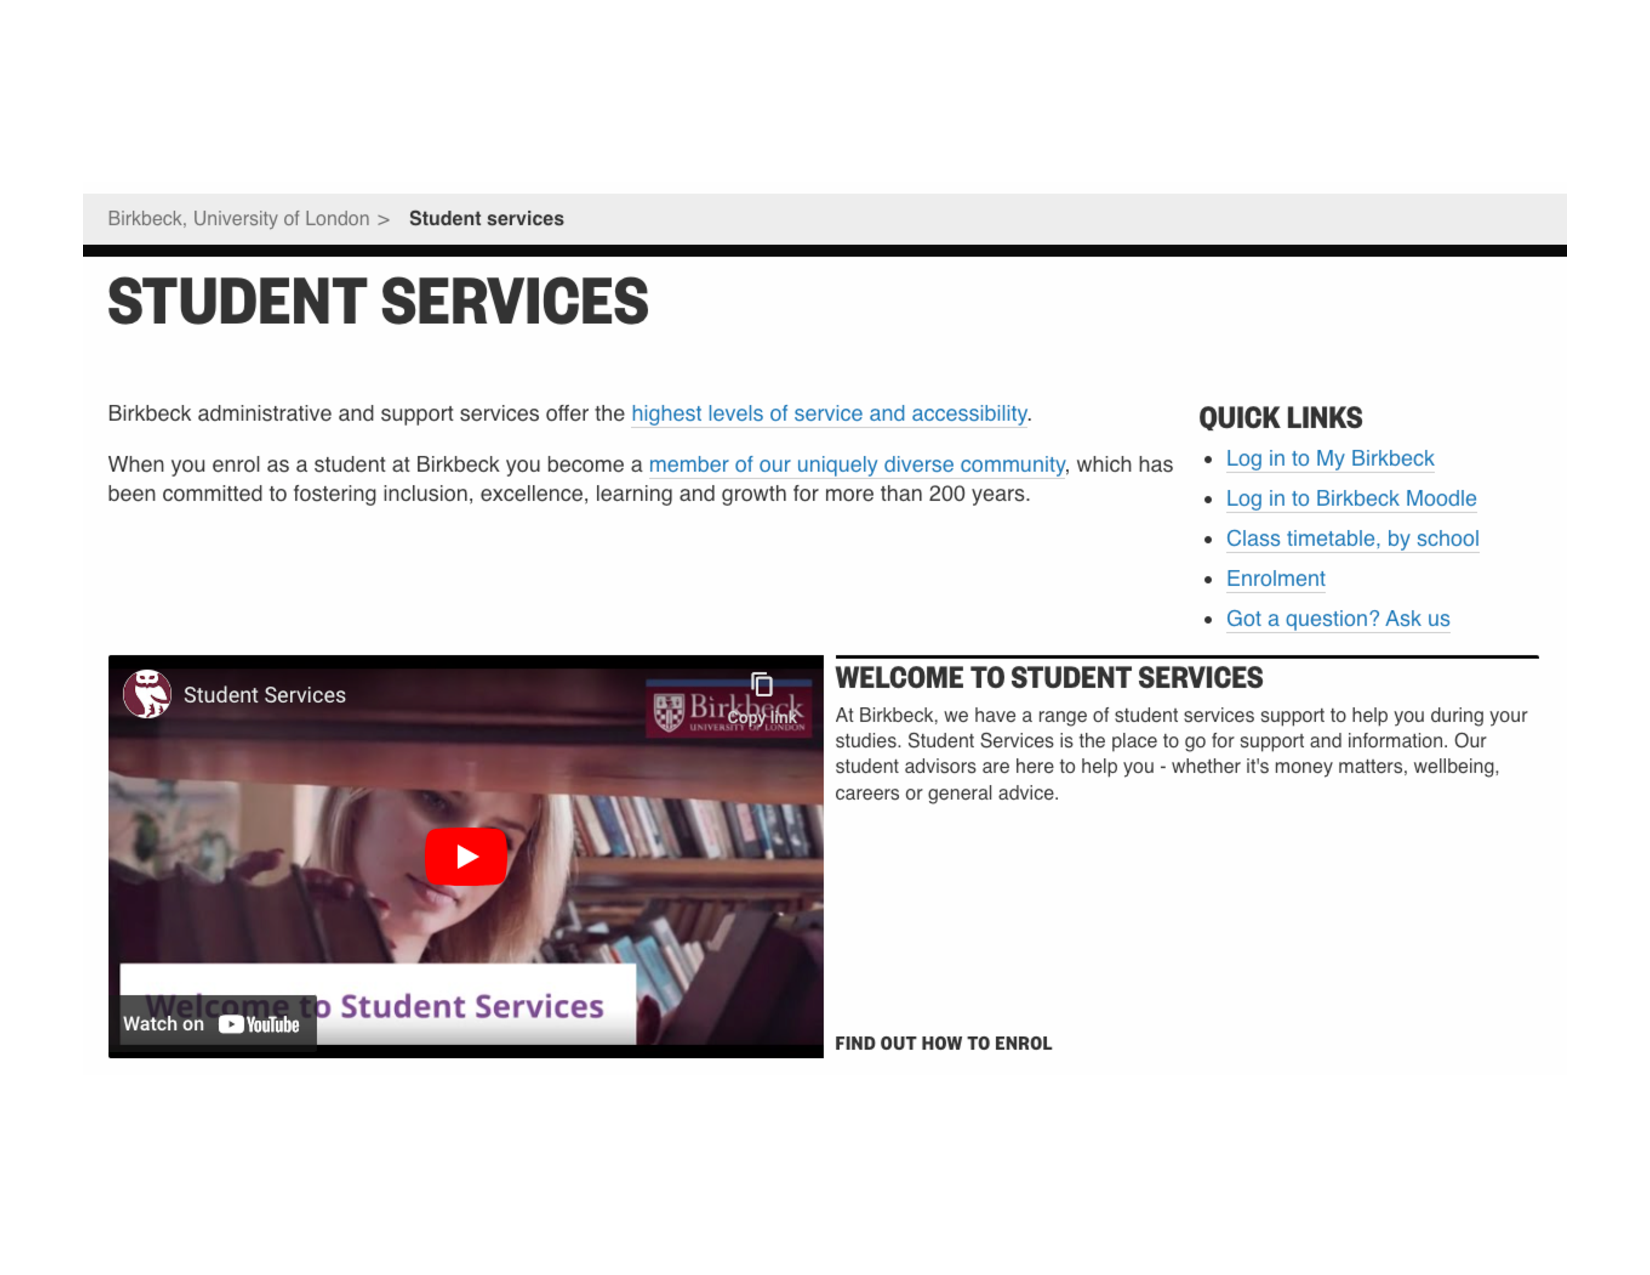
\includegraphics[width=1\linewidth]{Figs/student} \end{center}
\vspace{0.1cm}
\begin{center}
\url{https://www.bbk.ac.uk/student-services}
\end{center}
\end{frame}

\begin{frame}{Ground rules and tips}
\protect\hypertarget{ground-rules-and-tips}{}
\begin{itemize}
  \item \textbf{Active learning}: We embrace \textit{interactive} learning; come to in-person seminars/tutorials, having watched the lecture videos and completed the readings for the week
  \vspace{0.3cm}
  \item \textbf{Stability with flexibility}: We aim for stability, but acknowledge the need for flexibility
  \vspace{0.3cm}
  \item \textbf{Good communication}: We want to make this \textit{fantastic}; please be your own best advocate and give us feedback and constructive suggestions
  \vspace{0.3cm}
  \item \textbf{Safety}: We all want to keep you safe during your year at Birkbeck but need to work collaboratively with you to make that happen
\end{itemize}
\end{frame}

\begin{frame}{Strategic reading in social sciences}
\protect\hypertarget{strategic-reading-in-social-sciences}{}
\begin{itemize}
  \item Know why you are reading
  \vspace{0.1cm}
  \begin{itemize}
    \item Read the weekly description carefully
    \item Skim first before you dive in
    \item Pay attention to the big picture
    \item Find the key information and read closely
    \item Formulate your response and views
    \item Know there is always more to read (e.g., further readings)
  \end{itemize}
  \vspace{0.5cm}
  \item Build and use your support system
\end{itemize}
\end{frame}

\begin{frame}{Four-step approach (UC Berkeley)}
\protect\hypertarget{four-step-approach-uc-berkeley}{}
\vspace{0.2cm}

\begin{center}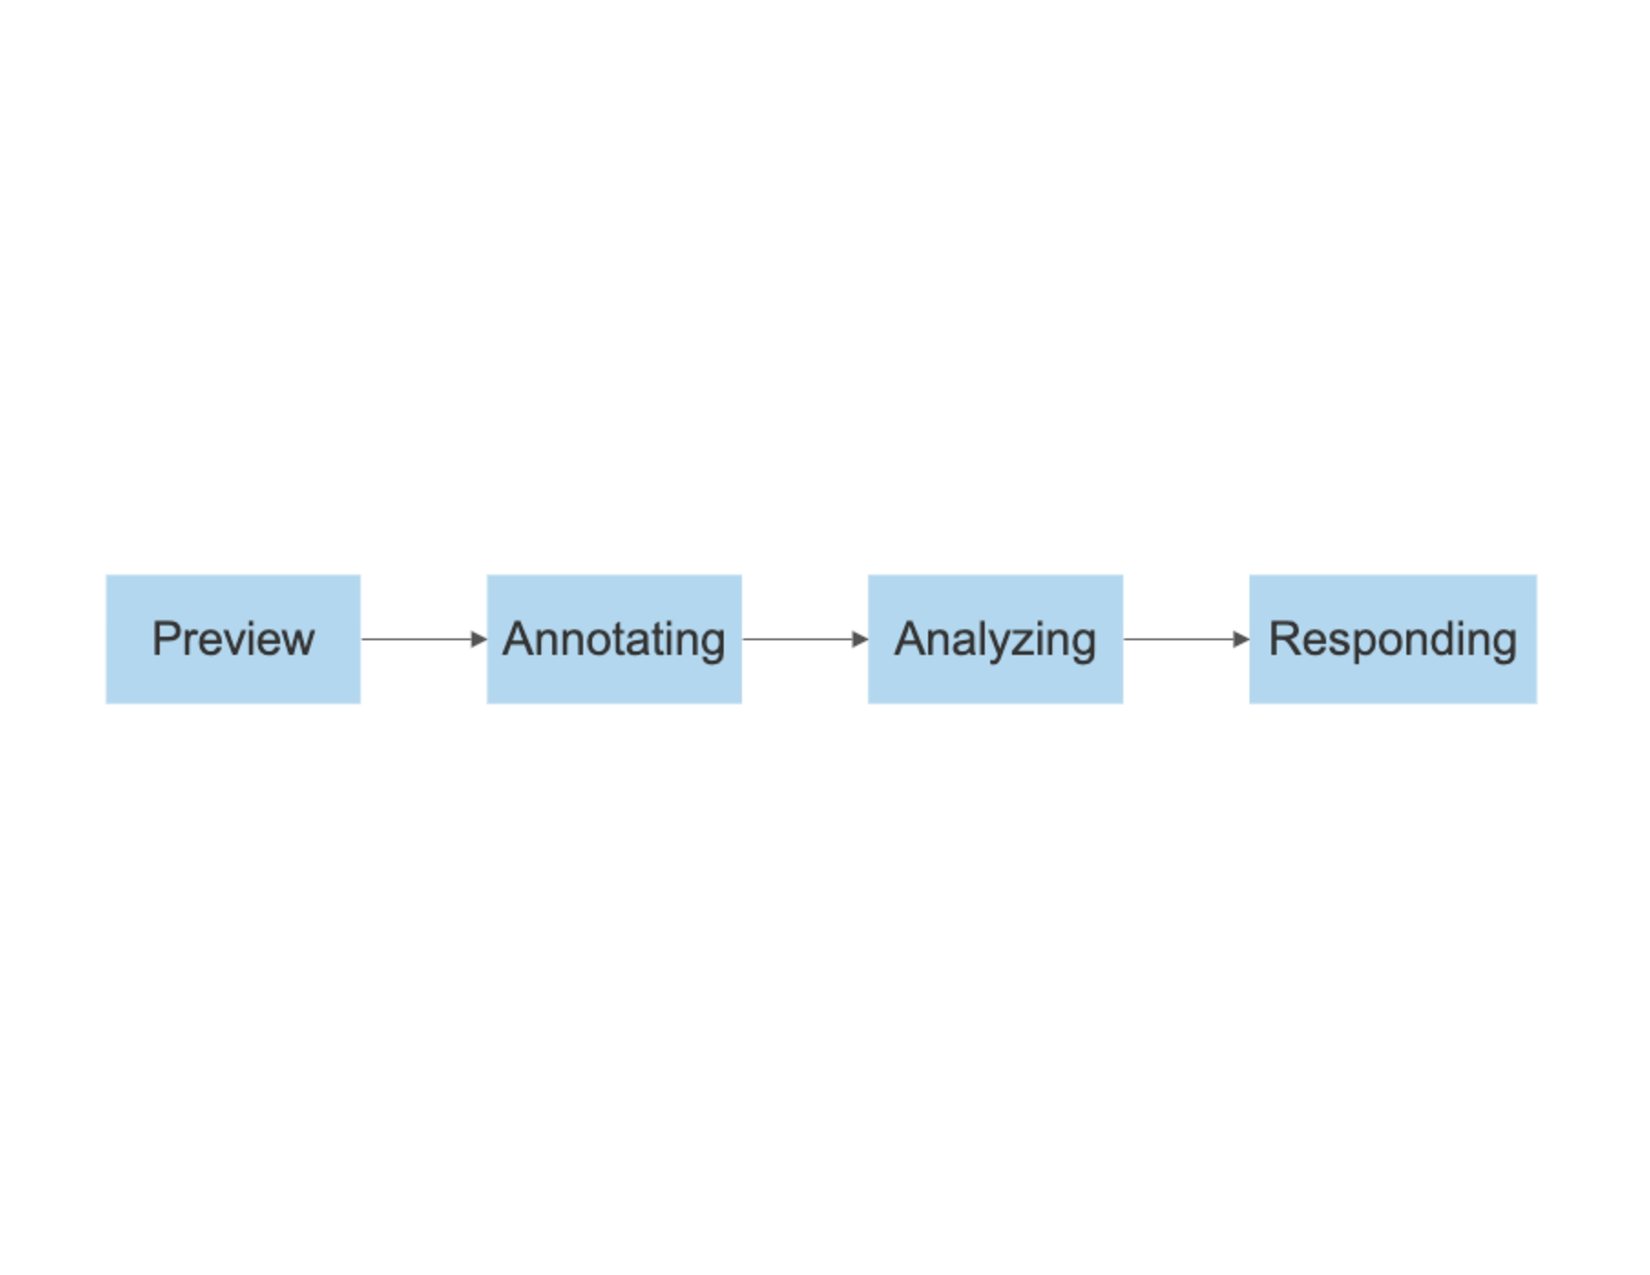
\includegraphics[width=1\linewidth]{Figs/ucb} \end{center}
\vspace{0.5cm}
\begin{itemize}
  \item \textbf{Preview}: Get as much information about the reading before you actually read it
  \vspace{0.1cm}
  \item \textbf{Annotating}: Read with a pencil and making notes as you read
  \vspace{0.1cm}
  \item \textbf{Analyzing}: Break the reading apart to see how different parts relate to each other
  \vspace{0.1cm}
  \item \textbf{Responding}: Think again how the reading relates the topic of each week; come up with questions
\end{itemize}
\end{frame}

\begin{frame}{Strategic reading in social sciences}
\protect\hypertarget{strategic-reading-in-social-sciences-1}{}
\begin{itemize}
  \item Know why you are reading
  \vspace{0.5cm}
  \item Build and use your support system
  \vspace{0.1cm}
  \begin{itemize}
    \item Study Skills workshops and online tutorials
    \item Personal/module tutor office hours
    \item Study clubs
  \end{itemize}
\end{itemize}
\end{frame}

\begin{frame}
\begin{center}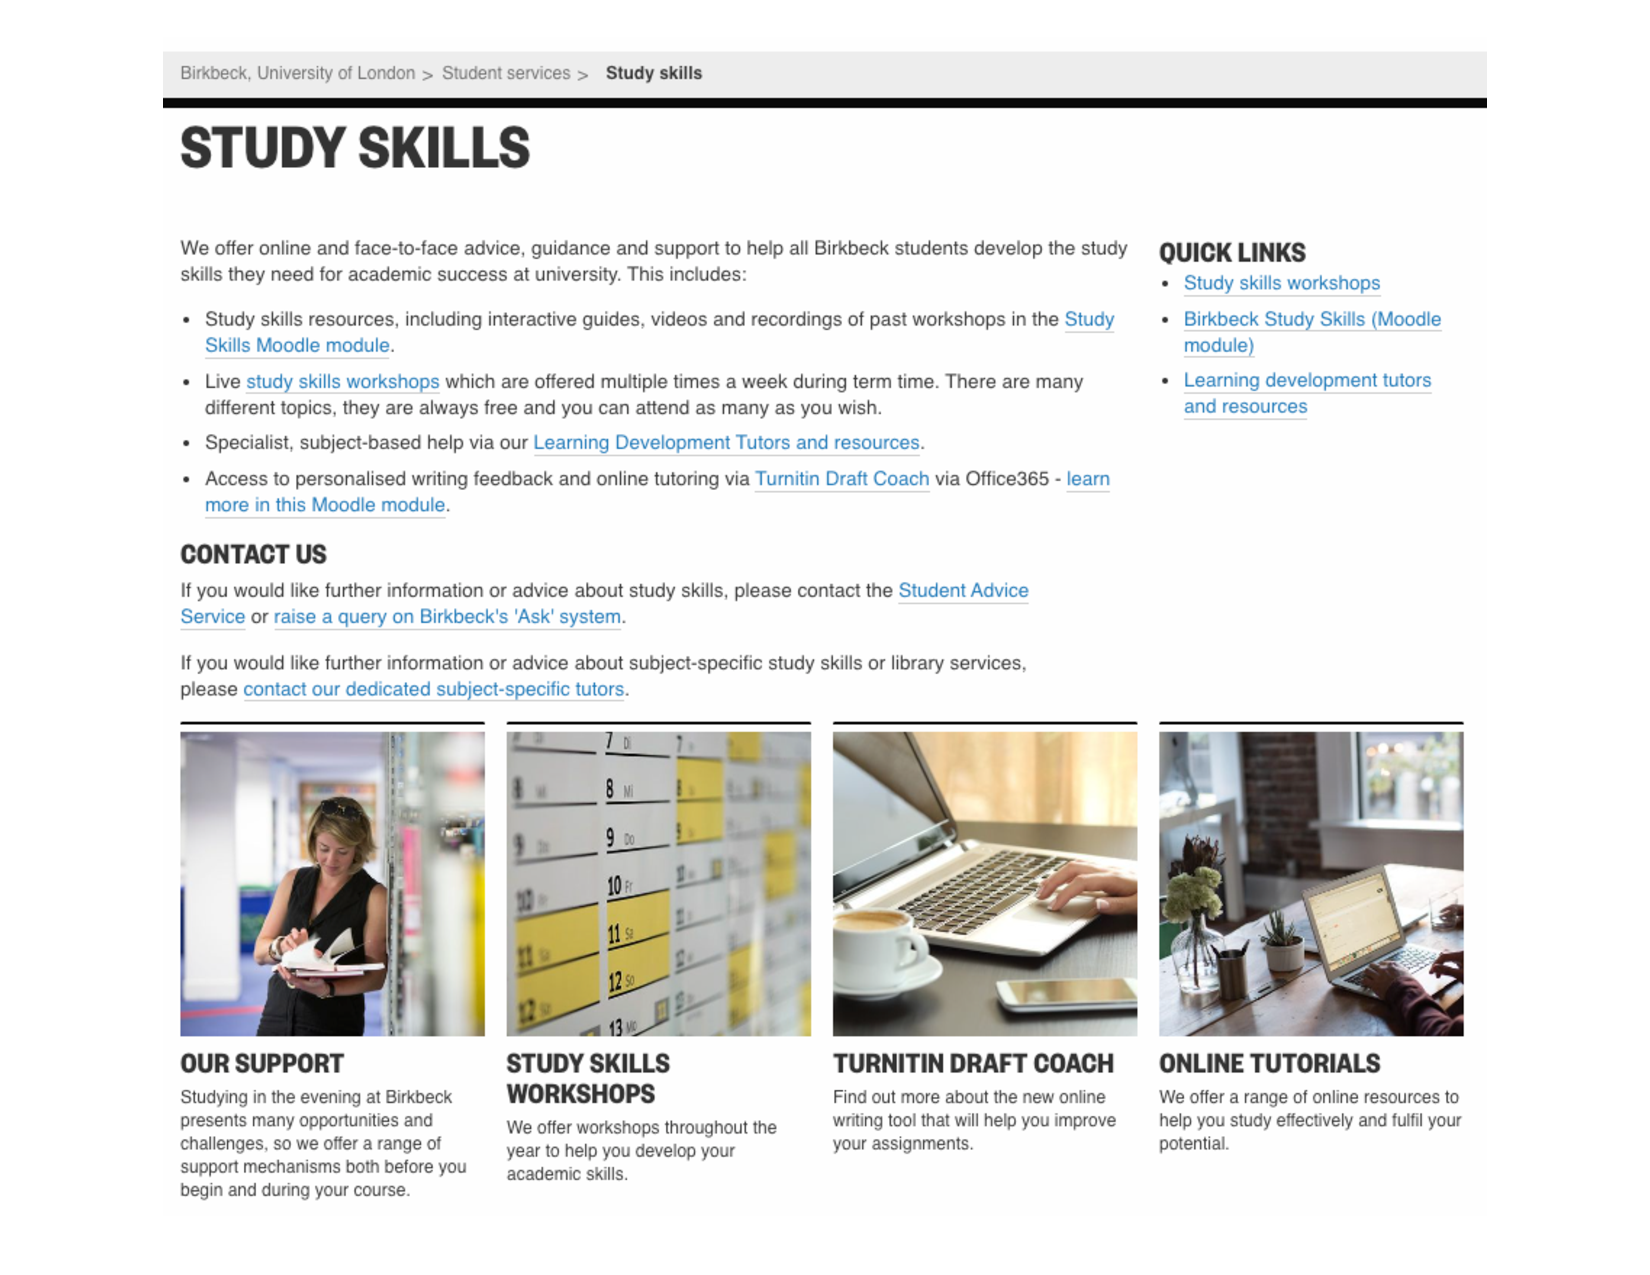
\includegraphics[width=0.9\linewidth]{Figs/study} \end{center}
\vspace{0.1cm}
\begin{center}
\url{https://www.bbk.ac.uk/student-services/learning-development}
\end{center}
\end{frame}

\begin{frame}{Breaking the ice: Humanities and social sciences in
crisis}
\protect\hypertarget{breaking-the-ice-humanities-and-social-sciences-in-crisis}{}
\begin{itemize}
  \item Social sciences as "pseudoscience?"
  \vspace{0.5cm}
  \item Debates over epistemological positions
  \vspace{0.5cm}
  \item Qualitative v quantitative? Or even computational?
  \vspace{0.5cm}
  \item Identity and representation -- how does "who you are" matter?
  \vspace{0.5cm}
  \item Replication, transparency and "open" social sciences
\end{itemize}
\end{frame}

\begin{frame}
\begin{center}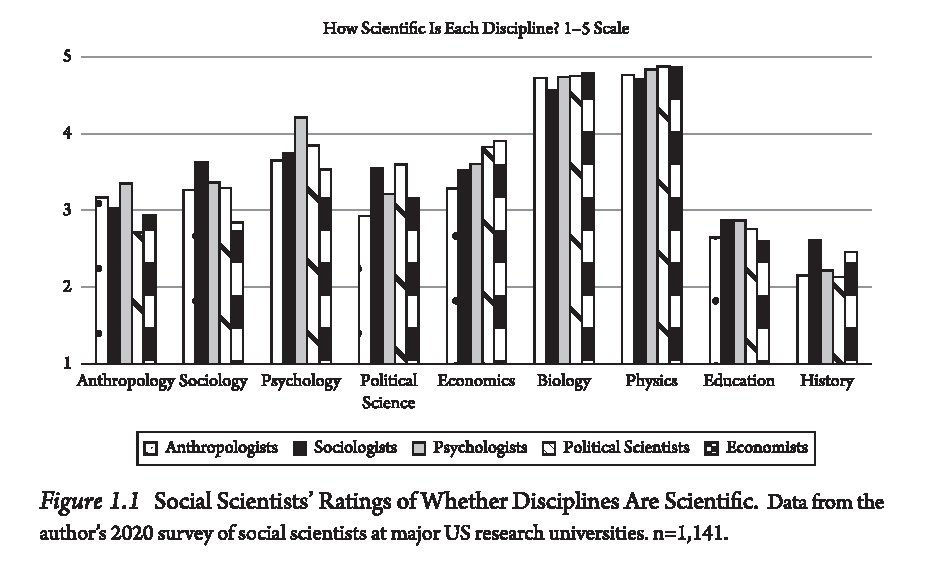
\includegraphics[width=1\linewidth]{Figs/subject_done} \end{center}
\end{frame}

\begin{frame}
\begin{center}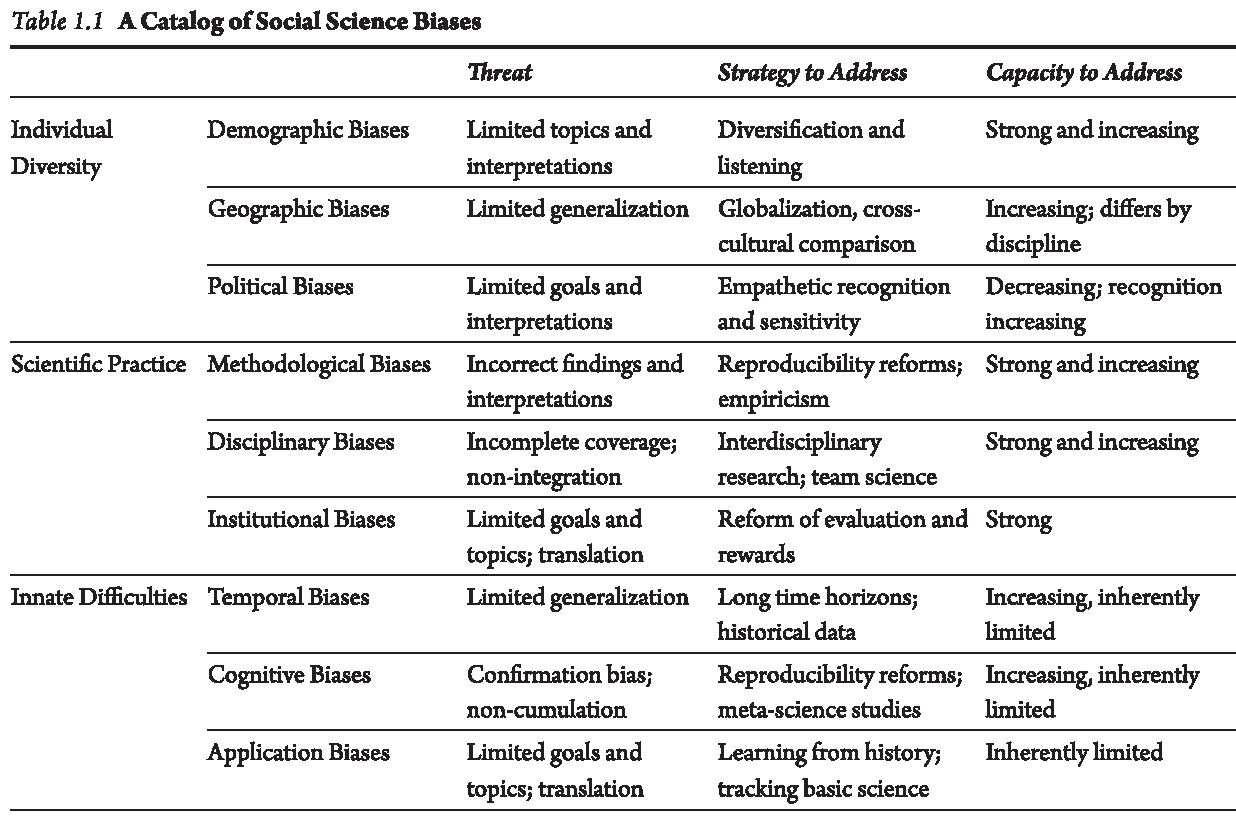
\includegraphics[width=1\linewidth]{Figs/biases_done} \end{center}
\end{frame}

\begin{frame}{Conclusion: Investigating the social world as a vocation}
\protect\hypertarget{conclusion-investigating-the-social-world-as-a-vocation}{}
\begin{itemize}
  \item ISW is a special module, reflecting on the production of "valid" knowledge about the social world
  \begin{itemize}
    \item You need to know what you do and how to explain the objectives of your scholarly inquiry;
    \item You need to know how to tell the differences between different objectives and engage other researchers' work constructively and effectively.
  \end{itemize}
  \item Social research involves a series of careful thinking about ontology/epistemology, theory-building, and methodology
  \begin{itemize}
    \item \textbf{Reveal nuances of the real world}: constructivism; theory as approach; interpretation; qualitative; inductive/abductive
    \item \textbf{Search for the "ultimate" truth}: positivism; theory as paradigm; explanation; quantitative; deductive
  \end{itemize}
  \item Paradigm shift and innovations: Boundaries are constantly being contested and redefined
\end{itemize}
\end{frame}

\begin{frame}
\begin{center}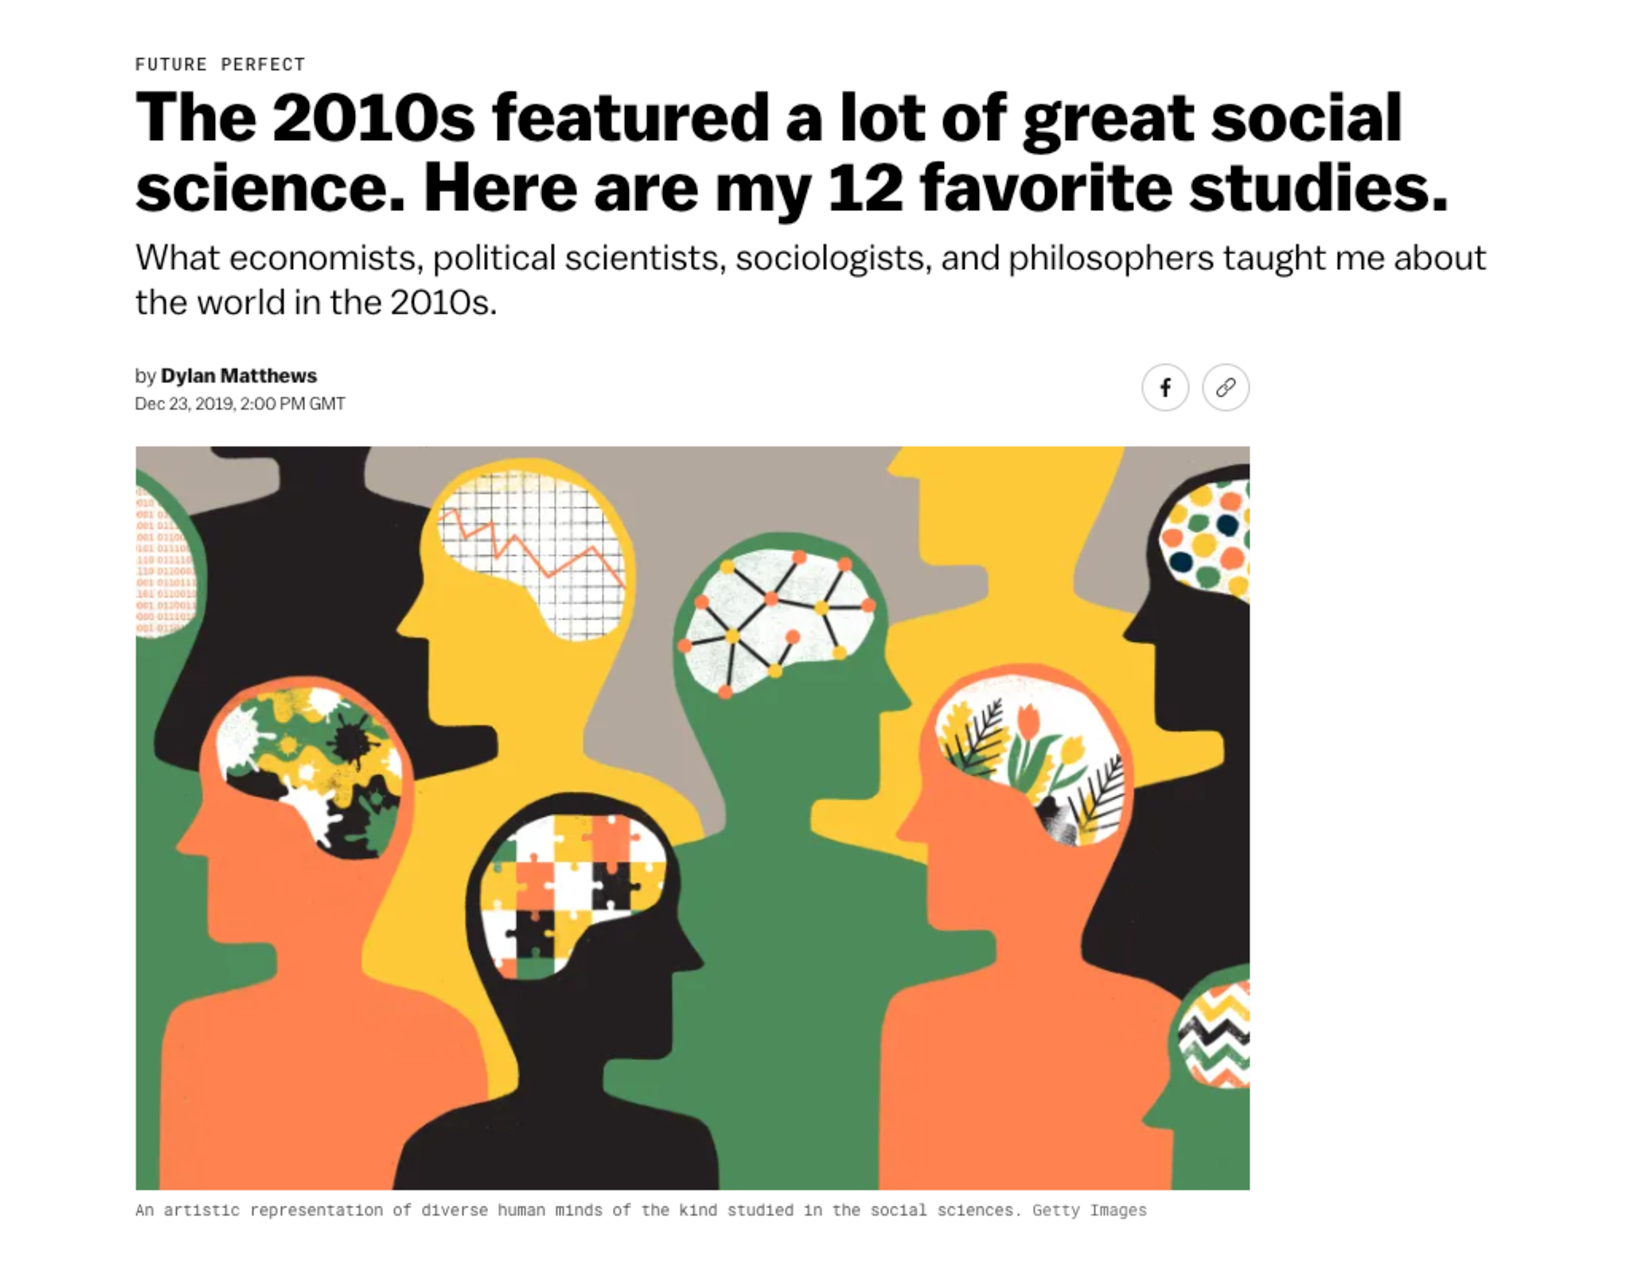
\includegraphics[width=0.95\linewidth]{Figs/vox} \end{center}
\end{frame}

\begin{frame}{Discussion}
\protect\hypertarget{discussion}{}
\begin{itemize}
  \item Which one of the 12 studies is your favorite, why?
  \vspace{0.3cm}
  \item What makes a social science research important? What makes a "good" social research?
  \vspace{0.3cm}
  \item We are now the fifth year into the 2020s, what are some of the topics that should (and can) be addressed by social researchers?
\end{itemize}
\end{frame}

\begin{frame}{Next week: Theory comes to rescue}
\protect\hypertarget{next-week-theory-comes-to-rescue}{}
\begin{center}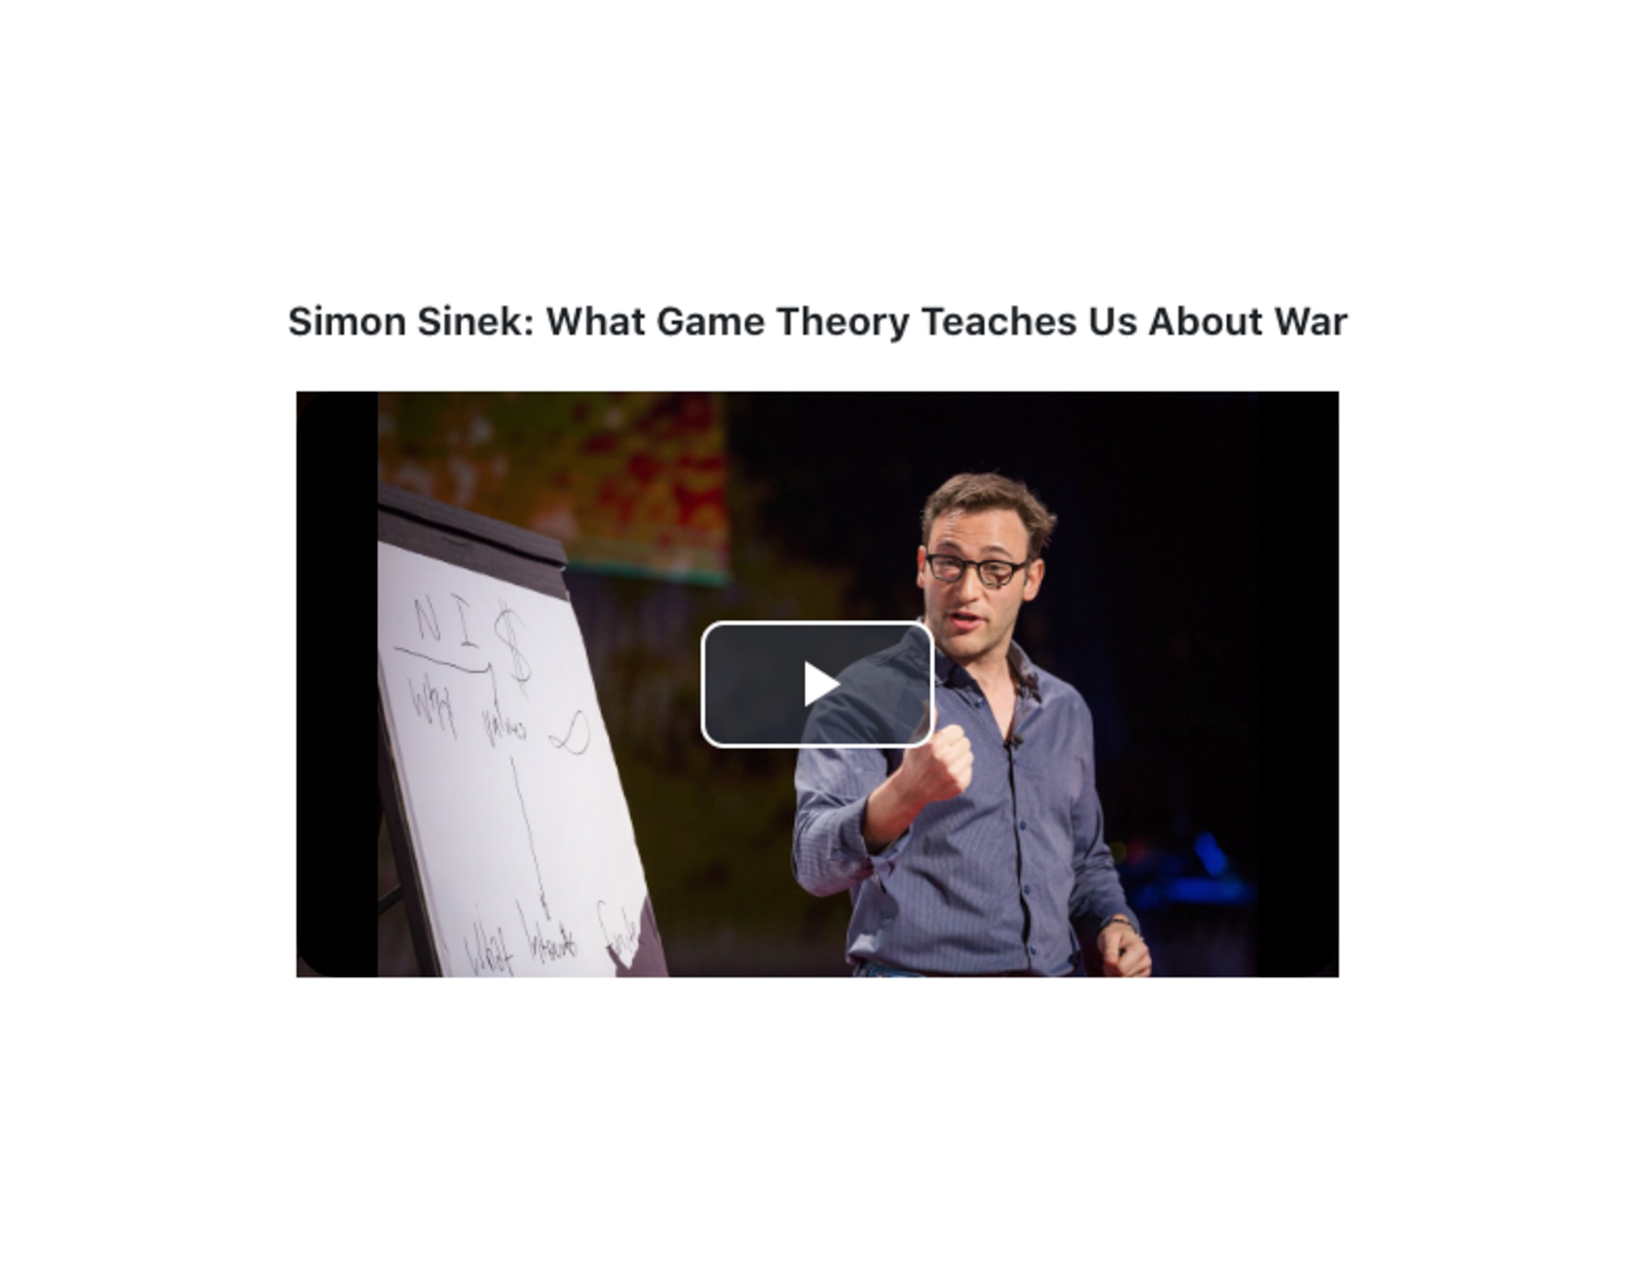
\includegraphics[width=0.7\linewidth]{Figs/simon} \end{center}
\begin{itemize}
\small
  \item Have you taken any module with "theory" in the title?
  \item What is the most important/famous theory in your subject area? And what makes it important/famous?
  \item What is your main takeaway from the TED Talk by Simon Sinek? Do you "like" what you hear (and does this matter)? Is there really a "theory" in the talk?
\end{itemize}
\end{frame}

\begin{frame}
\vspace{0.5cm}
\begin{center}
Thank you!
\end{center}
\vspace{0.3cm}

\begin{center}
\includegraphics[width=0.7\linewidth]{Figs/bbk_tv} \end{center}
\vspace{0.3cm}
\begin{center}
\texttt{c.cheng@bbk.ac.uk}
\end{center}
\end{frame}

\end{document}
